\documentclass[12pt]{article}
\usepackage[utf8]{inputenc}
\usepackage{graphicx}
\usepackage[table,xcdraw]{xcolor}
\graphicspath{{./}}

\title{assn2.3}
\author{
  Daniel Loi\\
  \texttt{dtloi@ucsc.edu}
  \texttt{1547401}
  \and
  Kevin Arellano\\
  \texttt{kcarella@ucsc.edu}
  \texttt{1550271}
  \and
  Claudio Sangeroki\\
  \texttt{csangero@ucsc.edu}
  \texttt{1677403}
}
\date{October 2019}

\begin{document}

\maketitle

\begin{enumerate}
    \item 
        \begin{enumerate}
        \item
        \[AI  = [70,75,80,85,85,90,100,150]\] 
        \[a  = [75,80,85,90,100,150]\] 
        Because AI is a continuous variable, we can partition it into ranges of the form AI $< a$ and AI $\geq a$, where $a$ is the midpoint between the AI[i], where AI[i] is the current value of AI we are considering, and AI[i+1] values. Therefore, if we have $N$ AI values, then we only need to consider $N-1$ partition values , or $a$ values. In this case, $N = 8$, $a = 7$.
        \item 
        Let $p_+ = P(B) = \frac{1}{2}$, $p_- = P(H) = \frac{1}{2}$, and $S = $ Preference. Therefore, 
        \[Entropy(S) = -\frac{1}{2}log_2(\frac{1}{2}) - \frac{1}{2}log_2(\frac{1}{2}) = 1\]
        \item 
        In order to find the optimal root, we will have to calculate the information gain between Gender vs. AI. 
            \begin{enumerate}
                \item In order to find out if we should split on Gender, we will calculate \[Gain(S, Gender) = E(S) - (E(S_1) + E(S_2))\] 
                where $S_1 = M$ and $S_2 = F$. 
                \[E(S_1) = -\frac{2}{3}log_2(\frac{2}{3}) - \frac{1}{3}log_2(\frac{1}{3}) = 0.91\]
                \[E(S_2) = -\frac{2}{5}log_2(\frac{2}{5}) - \frac{3}{5}log_2(\frac{3}{5}) = 0.97\]
                Therefore, 
                \[Gain(S, Gender) = 1 - ((\frac{3}{8})0.91 + (\frac{5}{8})0.97) = 0.0525\] 
                
                \item In order to find out if we should split on $a = 75$, we will calculate \[Gain(S, a) = E(S) - (E(S_1) + E(S_2))\] 
                where $S_1 = a < 75$ and $S_2 = a \geq 75$. 
                \[E(S_1) = -\frac{0}{1}log_2(\frac{0}{1}) - \frac{1}{1}log_2(\frac{1}{1}) = 0\]
                \[E(S_2) = -\frac{4}{7}log_2(\frac{4}{7}) - \frac{3}{7}log_2(\frac\frac{3}{7}) = 0.99\]
                Therefore, 
                \[Gain(S, a) = 1 - ((\frac{1}{8})0 + (\frac{7}{8})0.99) = 0.1338\] 
                
                \item In order to find out if we should split on $a = 80$, we will calculate \[Gain(S, a) = E(S) - (E(S_1) + E(S_2))\] 
                where $S_1 = a < 80$ and $S_2 = a \geq 80$. 
                \[E(S_1) = -\frac{1}{2}log_2(\frac{1}{2}) - \frac{1}{2}log_2(\frac{1}{2}) = 1\]
                \[E(S_2) = -\frac{1}{2}log_2(\frac{1}{2}) - \frac{1}{2}log_2(\frac{1}{2}) = 1\]
                Therefore, 
                \[Gain(S, a) = 1 - ((\frac{2}{8})1 + (\frac{6}{8})1) = 0\]
                
                \item In order to find out if we should split on $a = 85$, we will calculate \[Gain(S, a) = E(S) - (E(S_1) + E(S_2))\] 
                where $S_1 = a < 85$ and $S_2 = a \geq 85$. 
                \[E(S_1) = -\frac{2}{3}log_2(\frac{2}{3}) - \frac{1}{3}log_2(\frac{1}{3}) = 0.91\]
                \[E(S_2) = -\frac{2}{5}log_2(\frac{2}{5}) - \frac{3}{5}log_2(\frac{3}{5}) = 0.97\]
                Therefore, 
                \[Gain(S, a) = 1 - ((\frac{3}{8})0.91 + (\frac{5}{8})0.97) = 0.0525\] 
                
                
                \item In order to find out if we should split on $a = 90$, we will calculate \[Gain(S, a) = E(S) - (E(S_1) + E(S_2))\] 
                where $S_1 = a < 90$ and $S_2 = a \geq 90$. 
                \[E(S_1) = -\frac{2}{5}log_2(\frac{2}{5}) - \frac{3}{5}log_2(\frac{3}{5}) = 0.97\]
                \[E(S_2) = -\frac{2}{3}log_2(\frac{2}{3}) - \frac{1}{3}log_2(\frac{1}{3}) = 0.91\]
                Therefore, 
                \[Gain(S, a) = 1 - ((\frac{5}{8})0.97 + (\frac{3}{8})0.91) = 0.05250\]
                
                \item In order to find out if we should split on $a = 100$, we will calculate \[Gain(S, a) = E(S) - (E(S_1) + E(S_2))\] 
                where $S_1 = a < 100$ and $S_2 = a \geq 100$. 
                \[E(S_1) = -\frac{2}{6}log_2(\frac{2}{6}) - \frac{4}{6}log_2(\frac{4}{6}) = 0.91\]
                \[E(S_2) = -\frac{1}{1}log_2(\frac{1}{1}) - \frac{0}{1}log_2(\frac{0}{1}) = 0\]
                Therefore, 
                \[Gain(S, a) = 1 - ((\frac{6}{8})0.91 + (\frac{2}{8})0) = 0.3175\]
                
                \item In order to find out if we should split on $a = 150$, we will calculate \[Gain(S, a) = E(S) - (E(S_1) + E(S_2))\] 
                where $S_1 = a < 150$ and $S_2 = a \geq 150$. 
                \[E(S_1) = -\frac{3}{7}log_2(\frac{3}{7}) - \frac{4}{7}log_2(\frac{4}{7}) = 0.99\]
                \[E(S_2) = -\frac{0}{1}log_2(\frac{0}{1}) - \frac{1}{1}log_2(\frac{1}{1}) = 0\]
                Therefore, 
                \[Gain(S, a) = 1 - ((\frac{7}{8})0.99 + (\frac{1}{8})0) = 0.1338\]
                
            \end{enumerate}
            Since $a = 100$ gave us the highest information gain, it is the optimal root node to split on.
            
            \item 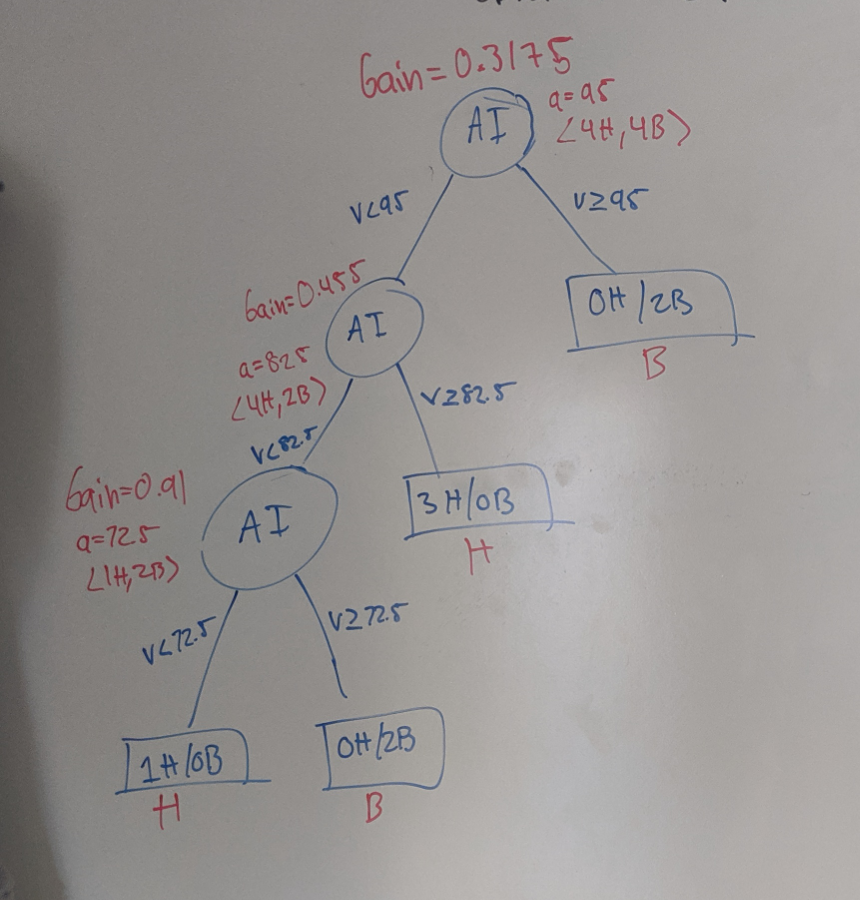
\includegraphics[width=9cm, height=10cm]{/DT.png}
            
            \item 
            \begin{table}[]
            \begin{tabular}{|l|l|l|}
            \hline
            Gender & AI  & Preference                        \\ \hline
            F      & 100 & B                                 \\ \hline
            M      & 150 & {\color[HTML]{FE0000} \textbf{H}} \\ \hline
            F      & 80  & B                                 \\ \hline
            M      & 75  & B                                 \\ \hline
            F      & 90  & H                                 \\ \hline
            F      & 85  & H                                 \\ \hline
            M      & 85  & H                                 \\ \hline
            F      & 70  & H                                 \\ \hline
            \end{tabular}
            \end{table}
            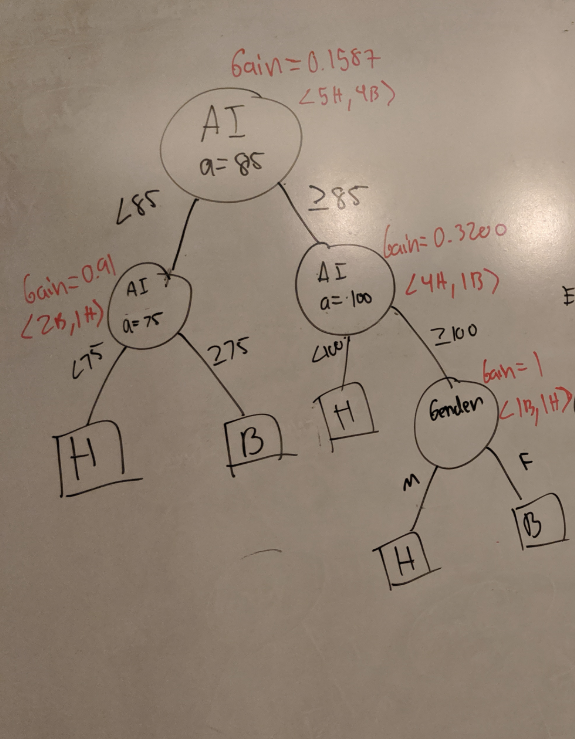
\includegraphics[width=9cm, height=10cm]{/DT2.png}
            
        \end{enumerate}
\end{enumerate}
    
\end{document}
